\documentclass[11pt]{beamer}
\usetheme{Warsaw}
\usepackage[utf8]{inputenc}
\usepackage[french]{babel}
\usepackage[T1]{fontenc}
\usepackage{amsmath}
\usepackage{amsfonts}
\usepackage{amssymb}
\usepackage{graphicx}
\usepackage{multirow}
\usepackage{color}
\author{Sarah Kaddah}
\title{Deciphering the function and evolution of the centromeric repeats in Primates}
\date{19/02/18} 
\institute{Tuteur: Loic Ponger\\
Département: Régulation, Développement, Diversité Moléculaire\\
Unité: Structure et Instabilité des génomes\\
CNRS UMR 7196 / INSERM U1154 / MNHN   
}
%\addtobeamertemplate{footline}{\hfill\insertframenumber/\inserttotalframenumber\hspace{2em}\null}

%\setbeamercovered{transparent} 
%\setbeamertemplate{navigation symbols}{} 
%\subject{} 
\begin{document}

%%%Diapo TITRE
\begin{frame}
\titlepage 
\end{frame}


%%%%%Table des matières%%%%%
%\begin{frame}
%\tableofcontents
%\end{frame}

%%%%%%%%%%%%%%%%%%%%%%%%%%%%%Diapo sur le centromere%%%%%%%%%%%%%%%%%%%%%%%%%%%%%%%%%%%%%%%
\begin{frame}{About the centromere}
	\begin{columns}
		%%%COL1
		\column{0.4\textwidth}
		\begin{itemize}
			\item Chromatin structure
			\item Cell division
			\item Conserved proteins 
			\item Not conserved DNA
				\begin{itemize}
				\item \textcolor{red}{\textbf{Satellite DNA}}
				\item Function ?
				\end{itemize}
		\end{itemize}
		%%%COL2
		\column{0.6\textwidth}
		\begin{figure}
			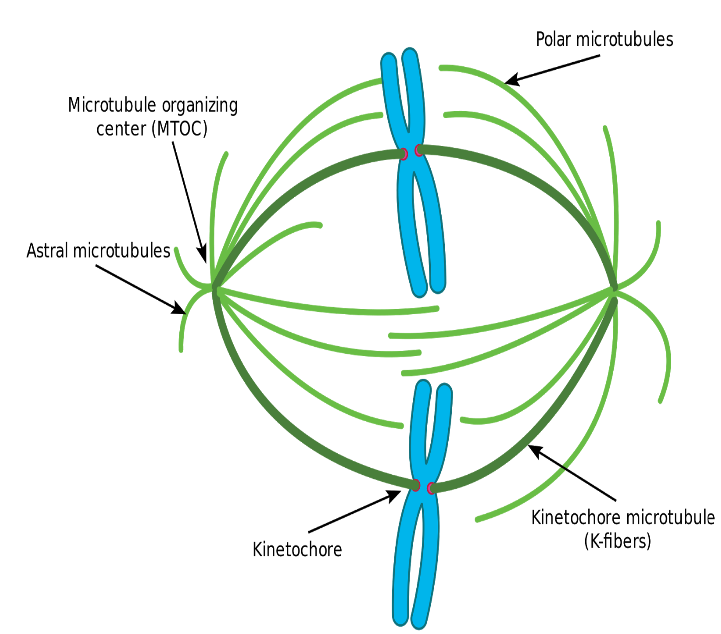
\includegraphics[width=\textwidth]{img/kinetochore.png}
		\end{figure}
		\begin{flushright}
			{\tiny Albert et al., 2002} 
		\end{flushright} 		
	\end{columns}
\logo{kkkk\tiny{\insertframenumber}}  

\end{frame}

%%%%%%%%%%%%%%%%%%%%%%%%%%%%%%%%%%ADN satellite chez le Primate%%%%%%%%%%%%%%%%%%%%%%%%%%%%%
\begin{frame}{Satellite DNA in Primates}
		\begin{itemize}
			\item \textcolor{red}{\textbf{$\alpha$-satellite}}
			\item  ~170 pb
			\item > 70\% similarity  
			\item Several families			
			\item Binding sites: CENP-B, pJ$\alpha$
			\item Specific spatial organisation
		\end{itemize}
		\begin{figure}
			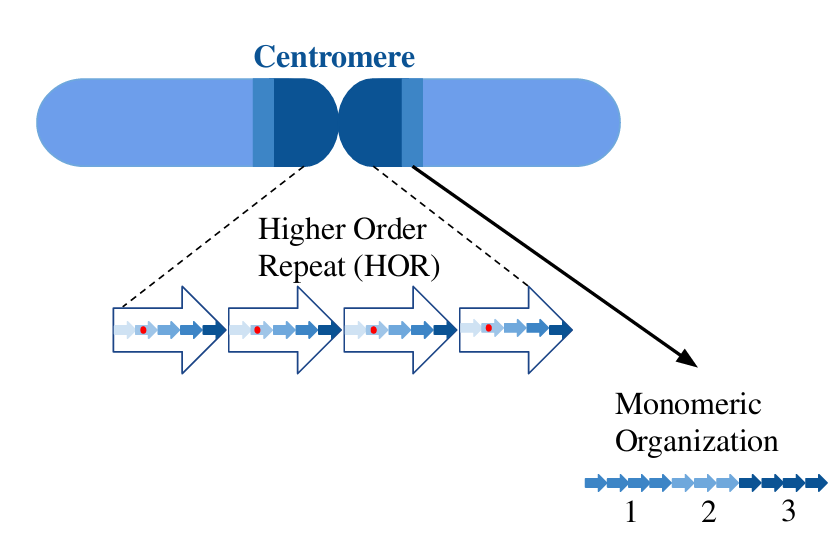
\includegraphics[width=0.7\textwidth]{img/AS_organization.png}
		\end{figure}	
\end{frame}

%%%%%%%%%%%%%%%%%%%%%%%%%Presentation des travaux deja effectues 1/2%%%%%%%%%%%%%%%%%%%%%%%
\begin{frame}{$\alpha$-satellites DNA}
	\begin{columns}	
		\column{0.4\textwidth}
		\textbf{Studies in human:}\\
		\medbreak
		Phylogenetic analysis of pericentromeric monomers\\
		\begin{itemize}
			\item Age-gradient hypothesis
			\item Identification of 5 families
		\end{itemize}		
		\column{0.6\textwidth}
		\begin{figure}
			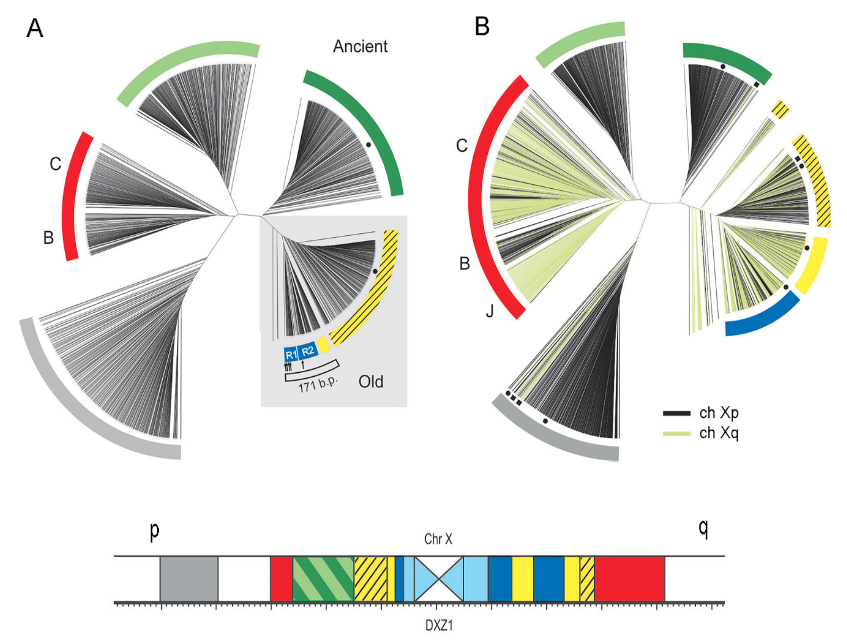
\includegraphics[width=\textwidth]{img/img_shepelev.png}
		\end{figure}
		\begin{flushright}
			{\tiny Shepelev et al., 2009} 
		\end{flushright}		
	\end{columns}
\end{frame}

%%%%%%%%%%%%%%%%%%%%%%%%%%%%%Presentation des travaux deja effectues 2/2%%%%%%%%%%%%%%%%%%%%
\begin{frame}{$\alpha$-satellites DNA}
	\begin{columns}
	%%%%%%%%%%%%COL1	
		\column{0.5\textwidth}
		\textbf{Studies on Gorillas:}\\
		{\tiny Catacchio et al., 2015}\\
		\begin{itemize}
			\item Medium throughput-sequencing
			\item Identification of 3 families 
			\item Complex HOR organization
			\item Binding sites for CENP-B and pJ$\alpha$
		\end{itemize}
		\textbf {Studies on Cercopithecini:}\\ 
		{\tiny Cacheux et al., 2016}\\
		\begin{itemize} 
			\item High throughput-sequencing
			\item Identification of 6 families
			\item Binding sites for pJ$\alpha$
		\end{itemize}	
		%%%%%%%%%%%%COL2	
		\column{0.5\textwidth}
		\begin{figure}
			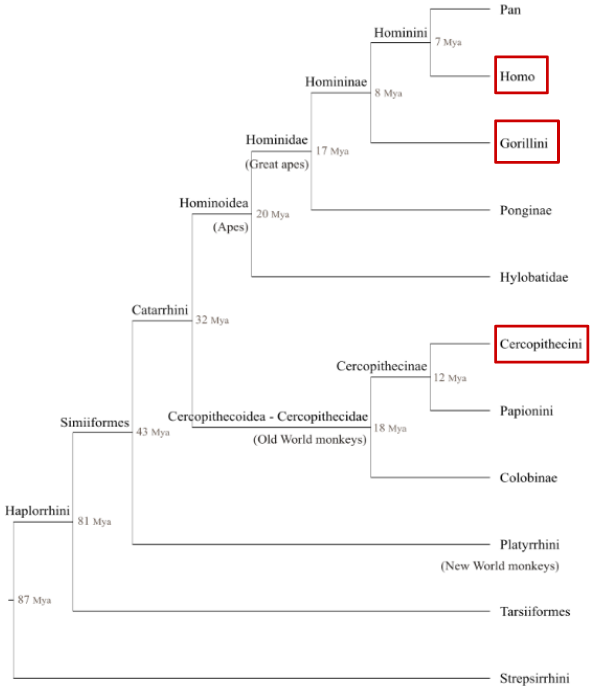
\includegraphics[width=\textwidth]{img/phylogenie_primates.png}
		\end{figure}	
		\begin{flushright}
			{\tiny Cacheux, Thèse} 
		\end{flushright}		
	\end{columns}
\end{frame}

%%%%%%%%%%%%%%%%%%%%%%%%%%%%%Partie 1%%%%%%%%%%%%%%%%%%%%
\begin{frame}{Goals}
\textbf{1- Choose species for analysis}

		\begin{center}
			% Tableau des données
			\medbreak						
			\begin{tabular}{|c|c|c|}
			\hline
			\begin{bf}Species\end{bf} & \begin{bf}\# of $\alpha$-sat.\end{bf} & \begin{bf}Sequencing\end{bf}\\
			\hline
			\textit{Cercopithecus pogonias} & 112 902 & Ion torrent\\
			\hline
			\textit{Cercopithecus solatus} & 105 529 & Ion torrent\\
			\hline
			\textit{Chlorocebus sabaeus} & 29 842 & Illumina\\
			\hline
			\textit{Macaca fascicularis} & 39 893 & LS454\\
			\hline
			\textit{Macaca fascicularis} & 195 642 & Assembly\\
			\hline			
			\end{tabular}										
		\end{center}
\end{frame}

%%%%%%%%%%%%%%%%%%%%%%%%%%%%%Partie 2 - méthode%%%%%%%%%%%%%%%%%%%%
\begin{frame}{Goals}
	1- Choose species for analysis \\ \medbreak
	\textbf{2 - Identify families for each species }\\ \medbreak
		\textbf{A-Method of classification}
		\begin{columns}	
		\column{0.5\textwidth}	
		\begin{itemize}
			\item Binary classification
			\item Objective and reproducible method
			\item Process big amount of short sequences
		\end{itemize}
		\column{0.5\textwidth}	
		\begin{figure}
			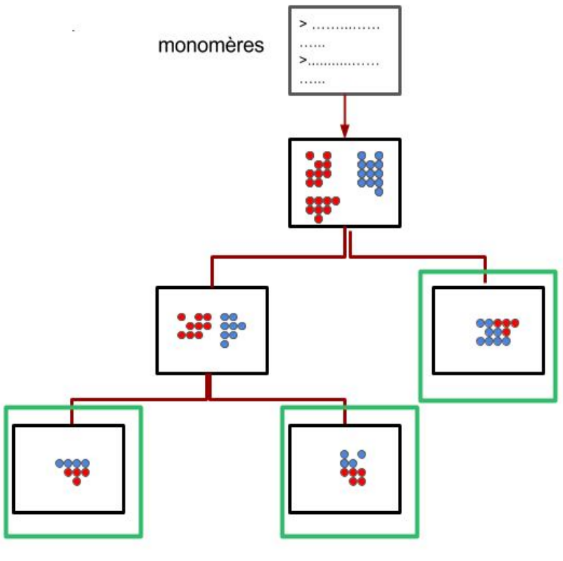
\includegraphics[width=0.7\textwidth]{img/algo_florence.png}
		\end{figure}	
		\end{columns}
		\begin{flushright}
			%{\tiny Jornod,2017 \\ Bridele, 2106}
			{\tiny Jornod,2017}
		\end{flushright} 
\end{frame}

%%%%%%%%%%%%%%%%%%%%%%%%Partie 2 - analyse%%%%%%%%%%%%%%%%
\begin{frame}{Goals}
	1- Choose species for analysis \\ \medbreak
	\textbf{2 - Identify families for each species } \\ \medbreak
	\textbf{B-Preliminary results}	
	\begin{figure}
		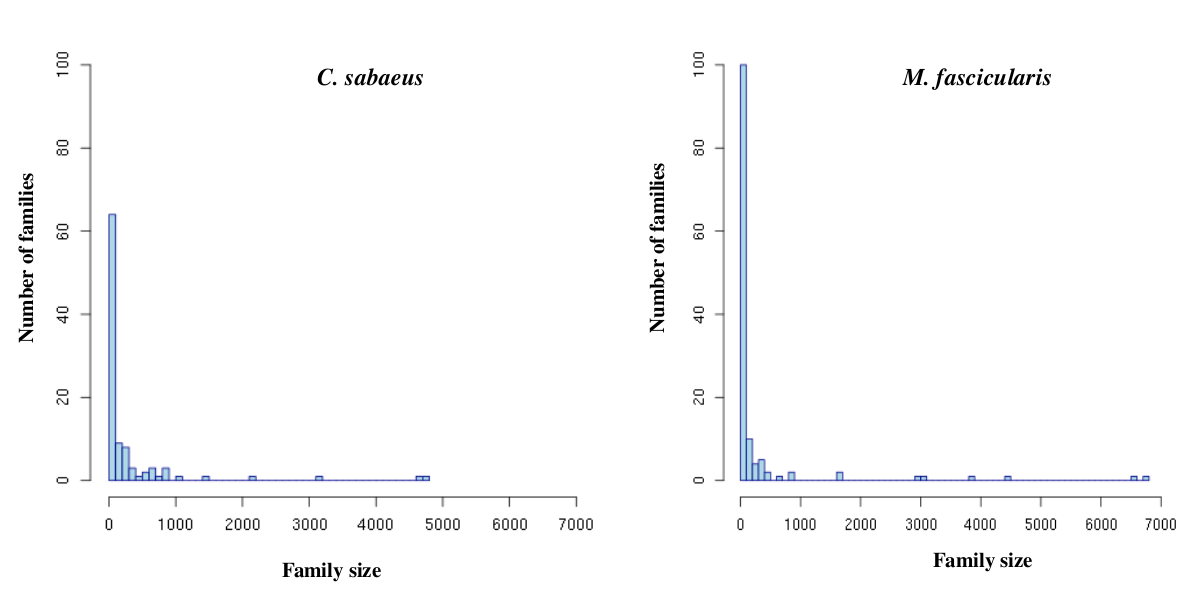
\includegraphics[width=\textwidth]{img/FamSize_NumFam2.png}
	\end{figure}	
\end{frame}

%%%%%%%%%%%%%%%%%%%%%%%%Diapos résultats avec tableau%%%%%%%%%%%%%%%%
\begin{frame}{Goals}
	1- Choose species for analysis \\ \medbreak
	\textbf{2 - Identify families for each species } \\ \medbreak
	\textbf{B-Results}

\begin{center}
			% Tableau des données
			\medbreak						
			\begin{tabular}{|c|c|c|}
			\hline
			\begin{bf}\end{bf} & \begin{bf}\textit{C. sabaeus}\end{bf} & \begin{bf}\textit{M. fascicularis}\end{bf}\\
			\hline
			\#Families & 100 & 132\\
			\hline
			\#Families > 100 sequences  & 36 & 32 \\
			\hline
			\% Sequences  & 95,3\% & 96,6\% \\
			\hline
			\end{tabular}			
		\end{center}
\end{frame}

%%%%%%%%%%%%%%%%%%%%%%%%Diapos presentation partie 3%%%%%%%%%%%%%%%%
\begin{frame}{Goals}

	1- Choose species for analysis \\ \medbreak
	2 - Identify families for each species \\ \medbreak
	\textbf{3 - Characterize families into each species}
		\begin{itemize}
			\item binding sites 
			\item percentage of similarity			 
		\end{itemize}
\end{frame}

%%%%%%%%%%%%%%%%%%%%%%%%Diapos MOTIF%%%%%%%%%%%%%%%%
%\begin{frame}{Workplan}
%	1- Choose species for analysis \\ \medbreak
%	2 - Identify families for each species \\ \medbreak
%	\textbf{3 - Characterize families into each species} \\ \medbreak
%	\textbf{A-Binding sites} \\ \medbreak	
%	\begin{center}
%			% Tableau des données
%			\medbreak						
%			\begin{tabular}{|c|c|c|c|}
%			\hline
%			\begin{bf}Binding site\end{bf} & \begin{bf}Condition\end{bf} & \begin{bf}\textit{C. sabaeus}\end{bf} & \begin{bf}\textit{M. fascicularis}\end{bf}\\
%			\hline					
%			\multirow{2}{*}{\textbf{CENP-B}} 			& \textbf{\% of seq.} & 0.007 & 0.005 \\			
%			\cline{2-4}
%			                        			& \textbf{\% of family} & 5.56   & 9.38\\
%			\hline					
%			\multirow{2}{*}{\textbf{pJ$\alpha$}}        	& \textbf{\% of seq.} & 0.47 & non \\
%			\cline{2-4}
%				 	            				& \textbf{\% of family} & 91.67 & 78,13\\
%			\hline
%			\end{tabular}			
%		\end{center}
%		\begin{flushright}
%			\tiny{\insertframenumber}
%		\end{flushright}
%\end{frame}


%%%%%%%%%%%%%%%%%%%%%%%%Diapos MOTIF schéma%%%%%%%%%%%%%%%%
\begin{frame}{Goals}
	1- Choose species for analysis \\ \medbreak
	2 - Identify families for each species \\ \medbreak
	\textbf{3 - Characterize families into each species} \\ \medbreak
	\textbf{A-Binding site} \\ 
		\begin{figure}
			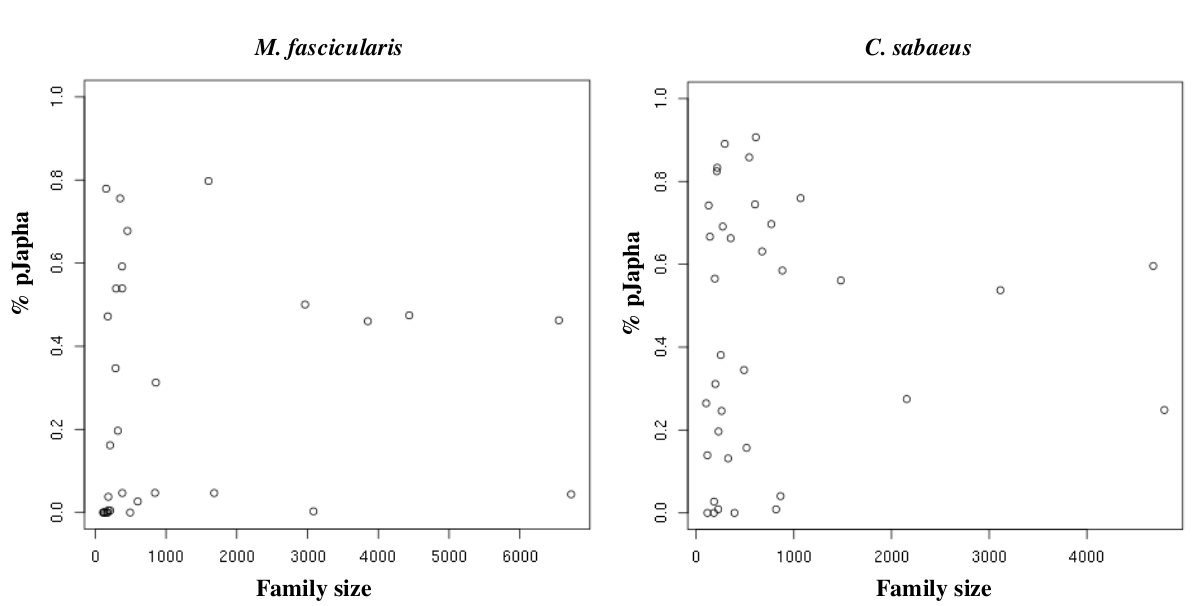
\includegraphics[width=\textwidth]{img/jpa.png}
		\end{figure}	
			\begin{flushright}
			\tiny{\insertframenumber}
		\end{flushright}
\end{frame}	

%%%%%%%%%%%%%%%%%%%%%%%%Diapos similarite%%%%%%%%%%%%%%%%
\begin{frame}{Goals}
	
	1- Choose species for analysis \\ \medbreak
	2 - Identify families for each species \\ \medbreak
	\textbf{3 - Characterize families into each species} \\ \medbreak
	\textbf{B-Similarity} \\ \medbreak
		\begin{figure}
			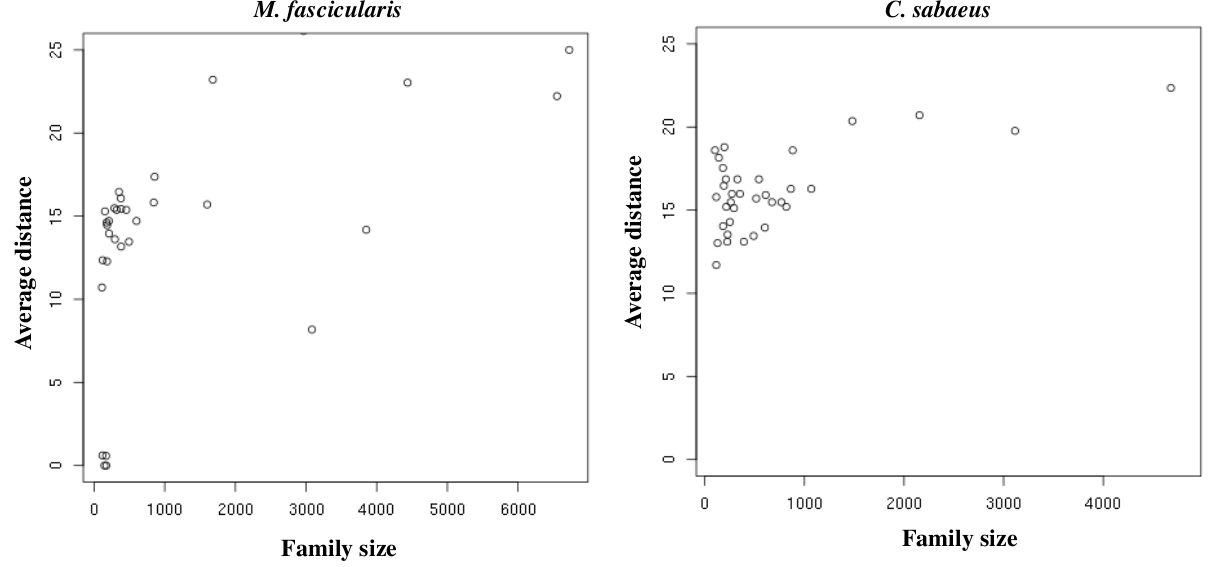
\includegraphics[width=\textwidth]{img/similarity_MF_CSA.png}
		\end{figure}
\end{frame}

%%%%%%%%%%%%%%%%%%%%%%%%Diapos cosnensus%%%%%%%%%%%%%%%%%%%%%%%%%%%
%\begin{frame}{Workplan}
%	1- Choose species for analysis \\ \medbreak
%	2 - Identify families for each species \\ \medbreak
%	\textbf{3 - Characterize families into each species} \\ \medbreak
%	\textbf{C-Consensus}
%\end{frame}
%%%%%%%%%%%%%%%%%%%%%%%%partie 4.1%%%%%%%%%%%%%%%%%%%%%%%%%%%
\begin{frame}{Goals}
	1- Choose species for analysis \\ \medbreak
	2 - Identify families for each species \\ \medbreak
	3 - Characterize families into each species \\ \medbreak
	\textbf{4 -1.  Spatial organization analysis} \\ \medbreak
		\begin{columns}
		\column{0.5\textwidth}
		\begin{figure}
			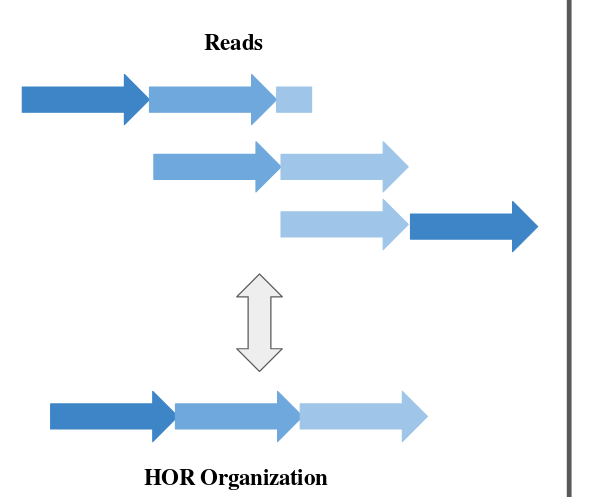
\includegraphics[width=\textwidth]{img/HOR.png}
		\end{figure}		
		\column{0.5\textwidth}	
		\begin{figure}
			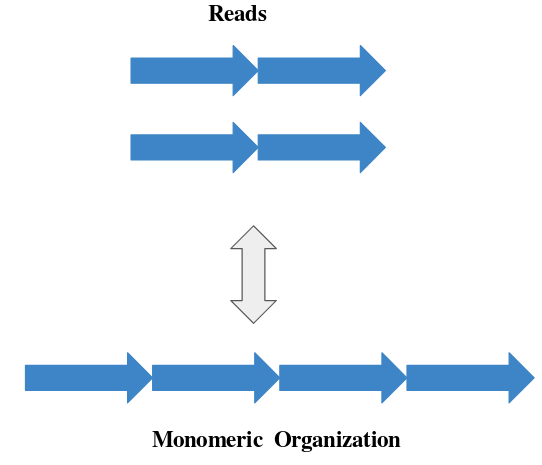
\includegraphics[width=\textwidth]{img/Monomeric_org.png}
		\end{figure}	
		\end{columns}	
	
	
	\begin{flushright}
		\tiny{\insertframenumber}
	\end{flushright}
\end{frame}
%%%%%%%%%%%%%%%%%%%%%%%%partie 4.2%%%%%%%%%%%%%%%%%%%%%%%%%%%
\begin{frame}{Goals}
	1- Choose species for analysis \\ \medbreak
	2 - Identify families for each species \\ \medbreak
	3 - Characterize families into each species \\ \medbreak
	4 -1.  Interspecific comparison \\ \medbreak
	\textbf{4 -2.  Interspecific comparison} \\ \medbreak
	\begin{figure}
		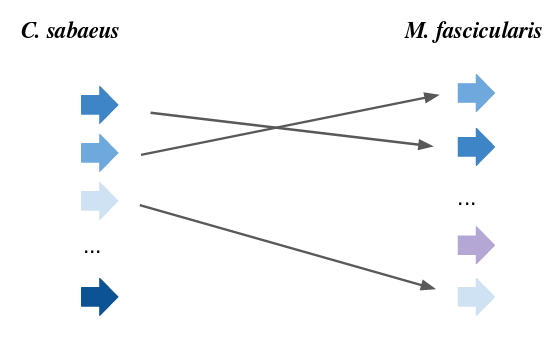
\includegraphics[width=0.5\textwidth]{img/comparaison_interespece.png}
	\end{figure}	
\end{frame}

%%%%%%Dans cette partie je montre ce qui a été fait%%%%%
%%%Presentation des données et choix de l'espèce
%\begin{frame}{Workplan}
%%%%%%%%%%%
%	\textbf <1> {1 - Choose species for analysis} \\ \medbreak
%		\only <1> {
%		\begin{center}
%			% Tableau des données
%			\medbreak						
%			\begin{tabular}{|c|c|}
%			\hline
%			\begin{bf}Species\end{bf} & \begin{bf}Sequences\end{bf} \\
%			\hline
%			Chlorocebus Sabaeus & 29842 \\
%			\hline
%			Macaca Fascicularis (SRA) & 39893 \\
%			\hline
%			Macaca Fascicularis (genome) & 195642 \\
%			\hline
%			Cercopithecus Pogonias & 112 902 \\
%			\hline
%			Cercopithecus Solatus & 105 529 \\
%			\hline
%			\end{tabular}			
%		\end{center}
%		}
%	\pause
%%%%%%%%%%%
%	\textbf <2> {2 - Identify families for each species }\\ \medbreak
%		\only <2> {
%		\begin{columns}	
%		\column{0.5\textwidth}	
%		\begin{itemize}
%			\item Objective and reproducible method
%			\item Process big amount of short sequences
%			\item Classification into families 
%			\item Binary classification
%		\end{itemize}
%		\column{0.5\textwidth}	
%		\begin{figure}
%			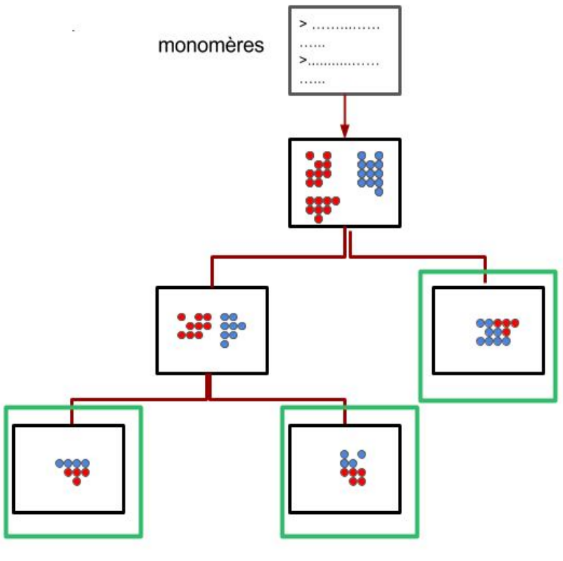
\includegraphics[width=0.7\textwidth]{img/algo_florence.png}
%		\end{figure}	
%		\end{columns}
%		}
%	\pause
%%%%%%%%%%%
%	\textbf <3, 4> {3 - Characterize families into each species} \\   \medbreak
%		\only <3> {
%		\begin{itemize}
%			\item percentage of similarity
%			\item binding sites...  
%		\end{itemize}
%		}
%		\temporal <4> {Salut je suis le temporal visible du slide 1} 
%%		\only <4> {
%%		\begin{columns}		
%%			\column{width=0.5\textwidth}
%%			Macaca fascicularis
%%			\begin{figure}
%%				\includegraphics[width=\textwidth]{../../results/Macaca_Fascicularis/img/similarity_n500_m100_d0_intra.png}
%%			\end{figure}
%%			\column{width=0.5\textwidth}
%%			Chlorocebus sabaeus
%%		\end{columns}
%%		}
%	\pause
%%%%%%%%%%%
%	\textbf <5> {4 -1.  Interspecific comparison} \\ \medbreak
%%%%%%%%%%%
%	\textbf <6> {4 -2.  Spatial organization analysis (HOR)}   \\ \medbreak
%	
%%	\pause
%%	\textbf <6> {5 - Writing of the report} \\ \medbreak
%
%\end{frame}

%%%%%%%%%%%%%%%%%%%%%%%Work in Progress%%%%%%%%%%%%%%%%%%%%%%%%%%%%%%
\begin{frame}
	\begin{center}
		\begin{figure}
			
\includegraphics[width=0.8\textwidth]{img/logo_work_in_progress2.jpg}
		\end{figure}	
	\end{center}
\end{frame}

%Dernière diapo
%\begin{frame}
%\begin{center}
%	\huge {Thank you for your attention !} 
%\end{center}
%\end{frame}

\end{document}